%--------------------
% Packages
% -------------------
\documentclass[11pt,english]{article}
\usepackage{amsfonts}
\usepackage[left=2.5cm,top=2cm,right=2.5cm,bottom=3cm,bindingoffset=0cm]{geometry}
\usepackage{amsmath, amsthm, amssymb}
\usepackage{tikz}
\usetikzlibrary{calc}
\usetikzlibrary{decorations.pathreplacing,calligraphy}
\usepackage{fancyhdr}
%\usepackage{currfile}
\usepackage{nicefrac}
\usepackage{cite}
\usepackage{graphicx}
\usepackage{caption}
\usepackage{longtable}
\usepackage{rotating}
\usepackage{lscape}
\usepackage{booktabs}
\usepackage{float}
\usepackage{placeins}
\usepackage{setspace}
\usepackage[font=itshape]{quoting}
\onehalfspacing
\usepackage{mathrsfs}
\usepackage{tcolorbox}
\usepackage{xcolor}
\usepackage{subcaption}
\usepackage{float}
\usepackage[multiple]{footmisc}
\usepackage[T1]{fontenc}
\usepackage[sc]{mathpazo}
\usepackage{listings}
\usepackage{longtable}
\definecolor{cmured}{RGB}{175,30,45}
\definecolor{macroblue}{RGB}{56,108,176}
\usepackage[format=plain,
            labelfont=bf,
            textfont=]{caption}
\usepackage[colorlinks=true,citecolor=macroblue,linkcolor=macroblue,urlcolor=macroblue]{hyperref}
\usepackage{varioref}
\usepackage{chngcntr}
\usepackage{datetime}

\definecolor{darkgreen}{RGB}{30,175,88}
\definecolor{darkblue}{RGB}{30,118,175}
\definecolor{maroon}{rgb}{0.66,0,0}
\definecolor{darkgreen}{rgb}{0,0.69,0}

%Counters
\newtheorem{theorem}{Theorem}[section] 
\newtheorem{proposition}{Proposition}
\newtheorem{lemma}{Lemma}
\newtheorem{corollary}{Corollary}
\newtheorem{assumption}{Assumption}
\newtheorem{axiom}{Axiom}
\newtheorem{case}{Case}
\newtheorem{claim}{Claim}
\newtheorem{condition}{Condition}
\newtheorem{definition}{Definition}
\newtheorem{example}{Example}
\newtheorem{notation}{Notation}
\newtheorem{remark}{Remark}


\hypersetup{ 	
pdfsubject = {},
pdftitle = {TidyTuesday Week 4},
pdfauthor = {Pranay Gundam},
linkcolor= macroblue
}


\title{\textbf{TidyTuesday Week 4}}
\author{Pranay Gundam}


%-----------------------
% Begin document
%-----------------------
\begin{document}

\maketitle

\tableofcontents

\section{Weekly Summary}


\section{Date: 2025-01-21}
\noindent \textbf{Series ID: DSBASEN} 

\noindent This series is titled St. Louis Source Base (DISCONTINUED) and has a frequency of Monthly. The units are Billions of Dollars and the seasonal adjustment is Not Seasonally Adjusted.The observation start date is 1936-01-01 and the observation end date is 2003-06-01.The popularity of this series is 1. \\ 

\noindent \textbf{Series ID: A2025C1A027NBEA} 

\noindent This series is titled Gross domestic product: Imputations: Financial services furnished without payment and has a frequency of Annual. The units are Billions of Dollars and the seasonal adjustment is Not Seasonally Adjusted.The observation start date is 1929-01-01 and the observation end date is 2022-01-01.The popularity of this series is 0. \\ 

\subsection{Regression Tables and Plots}
\begin{center}
\begin{tabular}{lclc}
\toprule
\textbf{Dep. Variable:}       & value\_fred\_A2025C1A027NBEA & \textbf{  R-squared:         } &     0.879   \\
\textbf{Model:}               &             OLS              & \textbf{  Adj. R-squared:    } &     0.877   \\
\textbf{Method:}              &        Least Squares         & \textbf{  F-statistic:       } &     478.9   \\
\textbf{Date:}                &       Tue, 21 Jan 2025       & \textbf{  Prob (F-statistic):} &  5.80e-32   \\
\textbf{Time:}                &           09:31:01           & \textbf{  Log-Likelihood:    } &   -261.78   \\
\textbf{No. Observations:}    &                68            & \textbf{  AIC:               } &     527.6   \\
\textbf{Df Residuals:}        &                66            & \textbf{  BIC:               } &     532.0   \\
\textbf{Df Model:}            &                 1            & \textbf{                     } &             \\
\textbf{Covariance Type:}     &          nonrobust           & \textbf{                     } &             \\
\bottomrule
\end{tabular}
\begin{tabular}{lcccccc}
                              & \textbf{coef} & \textbf{std err} & \textbf{t} & \textbf{P$> |$t$|$} & \textbf{[0.025} & \textbf{0.975]}  \\
\midrule
\textbf{const}                &       0.8980  &        1.914     &     0.469  &         0.640        &       -2.923    &        4.719     \\
\textbf{value\_fred\_DSBASEN} &       0.1736  &        0.008     &    21.885  &         0.000        &        0.158    &        0.189     \\
\bottomrule
\end{tabular}
\begin{tabular}{lclc}
\textbf{Omnibus:}       &  9.077 & \textbf{  Durbin-Watson:     } &    0.145  \\
\textbf{Prob(Omnibus):} &  0.011 & \textbf{  Jarque-Bera (JB):  } &    9.473  \\
\textbf{Skew:}          &  0.658 & \textbf{  Prob(JB):          } &  0.00877  \\
\textbf{Kurtosis:}      &  4.269 & \textbf{  Cond. No.          } &     330.  \\
\bottomrule
\end{tabular}
%\caption{OLS Regression Results}
\end{center}

Notes: \newline
 [1] Standard Errors assume that the covariance matrix of the errors is correctly specified.

\begin{figure}
\centering
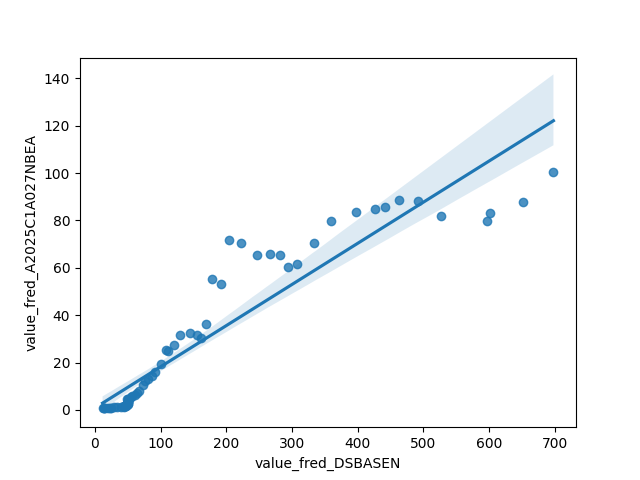
\includegraphics[scale = 0.9]{plots/plot_2025-01-21.png}
\caption{Regression Plot for 2025-01-21}
\end{figure}
\newpage

\section{Date: 2025-01-22}
\noindent \textbf{Series ID: NCBCBIA027N} 

\noindent This series is titled Nonfinancial Corporate Business; Corporate Bonds; Liability (Excluding eREITs), Level and has a frequency of Annual. The units are Millions of Dollars and the seasonal adjustment is Not Seasonally Adjusted.The observation start date is 1945-01-01 and the observation end date is 2023-01-01.The popularity of this series is 4. \\ 

\noindent \textbf{Series ID: MDOTHMPTFAMCTPFP} 

\noindent This series is titled Mortgage Debt Outstanding by Type of Holder and Property: Mortgage Pools or Trust: Federal Agricultural Mortgage Corporation for Farm Properties (DISCONTINUED) and has a frequency of Quarterly, End of Period. The units are Millions of Dollars and the seasonal adjustment is Not Seasonally Adjusted.The observation start date is 1949-01-01 and the observation end date is 2019-07-01.The popularity of this series is 2. \\ 

\subsection{Regression Tables and Plots}
\begin{center}
\begin{tabular}{lclc}
\toprule
\textbf{Dep. Variable:}           & value\_fred\_MDOTHMPTFAMCTPFP & \textbf{  R-squared:         } &     0.589   \\
\textbf{Model:}                   &              OLS              & \textbf{  Adj. R-squared:    } &     0.583   \\
\textbf{Method:}                  &         Least Squares         & \textbf{  F-statistic:       } &     99.01   \\
\textbf{Date:}                    &        Wed, 22 Jan 2025       & \textbf{  Prob (F-statistic):} &  5.72e-15   \\
\textbf{Time:}                    &            14:49:53           & \textbf{  Log-Likelihood:    } &   -567.32   \\
\textbf{No. Observations:}        &                 71            & \textbf{  AIC:               } &     1139.   \\
\textbf{Df Residuals:}            &                 69            & \textbf{  BIC:               } &     1143.   \\
\textbf{Df Model:}                &                  1            & \textbf{                     } &             \\
\textbf{Covariance Type:}         &           nonrobust           & \textbf{                     } &             \\
\bottomrule
\end{tabular}
\begin{tabular}{lcccccc}
                                  & \textbf{coef} & \textbf{std err} & \textbf{t} & \textbf{P$> |$t$|$} & \textbf{[0.025} & \textbf{0.975]}  \\
\midrule
\textbf{const}                    &    -104.4915  &      113.162     &    -0.923  &         0.359        &     -330.243    &      121.260     \\
\textbf{value\_fred\_NCBCBIA027N} &       0.0005  &      5.3e-05     &     9.951  &         0.000        &        0.000    &        0.001     \\
\bottomrule
\end{tabular}
\begin{tabular}{lclc}
\textbf{Omnibus:}       & 55.828 & \textbf{  Durbin-Watson:     } &    0.419  \\
\textbf{Prob(Omnibus):} &  0.000 & \textbf{  Jarque-Bera (JB):  } &  252.960  \\
\textbf{Skew:}          &  2.389 & \textbf{  Prob(JB):          } & 1.18e-55  \\
\textbf{Kurtosis:}      & 10.917 & \textbf{  Cond. No.          } & 2.81e+06  \\
\bottomrule
\end{tabular}
%\caption{OLS Regression Results}
\end{center}

Notes: \newline
 [1] Standard Errors assume that the covariance matrix of the errors is correctly specified. \newline
 [2] The condition number is large, 2.81e+06. This might indicate that there are \newline
 strong multicollinearity or other numerical problems.

\begin{figure}
\centering
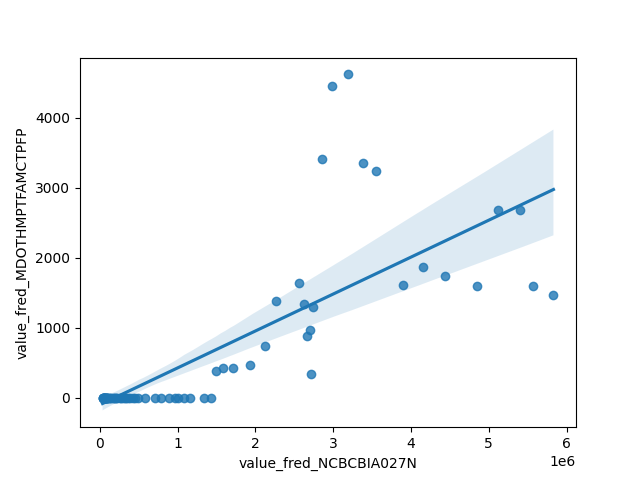
\includegraphics[scale = 0.9]{plots/plot_2025-01-22.png}
\caption{Regression Plot for 2025-01-22}
\end{figure}
\newpage

\section{Date: 2025-01-23}
\noindent \textbf{Series ID: LNU03023654} 

\noindent This series is titled Job Losers on Layoff as a Percent of Total Unemployed and has a frequency of Monthly. The units are Percent and the seasonal adjustment is Not Seasonally Adjusted.The observation start date is 1967-01-01 and the observation end date is 2024-12-01.The popularity of this series is 2. \\ 

\noindent \textbf{Series ID: ATLSBUEGEI} 

\noindent This series is titled Business Expectations: Employment Growth Index (DISCONTINUED) and has a frequency of Monthly. The units are Index and the seasonal adjustment is Not Seasonally Adjusted.The observation start date is 2015-01-01 and the observation end date is 2020-07-01.The popularity of this series is 2. \\ 

\subsection{Regression Tables and Plots}
\begin{center}
\begin{tabular}{lclc}
\toprule
\textbf{Dep. Variable:}           & value\_fred\_ATLSBUEGEI & \textbf{  R-squared:         } &     0.055   \\
\textbf{Model:}                   &           OLS           & \textbf{  Adj. R-squared:    } &     0.040   \\
\textbf{Method:}                  &      Least Squares      & \textbf{  F-statistic:       } &     3.780   \\
\textbf{Date:}                    &     Thu, 23 Jan 2025    & \textbf{  Prob (F-statistic):} &   0.0562    \\
\textbf{Time:}                    &         15:38:04        & \textbf{  Log-Likelihood:    } &   -241.05   \\
\textbf{No. Observations:}        &              67         & \textbf{  AIC:               } &     486.1   \\
\textbf{Df Residuals:}            &              65         & \textbf{  BIC:               } &     490.5   \\
\textbf{Df Model:}                &               1         & \textbf{                     } &             \\
\textbf{Covariance Type:}         &        nonrobust        & \textbf{                     } &             \\
\bottomrule
\end{tabular}
\begin{tabular}{lcccccc}
                                  & \textbf{coef} & \textbf{std err} & \textbf{t} & \textbf{P$> |$t$|$} & \textbf{[0.025} & \textbf{0.975]}  \\
\midrule
\textbf{const}                    &     102.5163  &        1.734     &    59.124  &         0.000        &       99.053    &      105.979     \\
\textbf{value\_fred\_LNU03023654} &      -0.1589  &        0.082     &    -1.944  &         0.056        &       -0.322    &        0.004     \\
\bottomrule
\end{tabular}
\begin{tabular}{lclc}
\textbf{Omnibus:}       &  6.964 & \textbf{  Durbin-Watson:     } &    0.263  \\
\textbf{Prob(Omnibus):} &  0.031 & \textbf{  Jarque-Bera (JB):  } &    3.712  \\
\textbf{Skew:}          &  0.359 & \textbf{  Prob(JB):          } &    0.156  \\
\textbf{Kurtosis:}      &  2.098 & \textbf{  Cond. No.          } &     33.6  \\
\bottomrule
\end{tabular}
%\caption{OLS Regression Results}
\end{center}

Notes: \newline
 [1] Standard Errors assume that the covariance matrix of the errors is correctly specified.

\begin{figure}
\centering
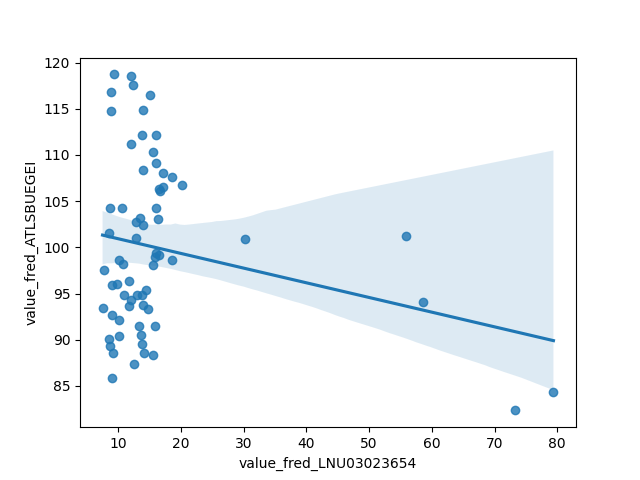
\includegraphics[scale = 0.9]{plots/plot_2025-01-23.png}
\caption{Regression Plot for 2025-01-23}
\end{figure}
\newpage

\section{Date: 2025-01-24}
\noindent \textbf{Series ID: EAAMNQ} 

\noindent This series is titled Average Loan Size for All Commercial and Industry Loans, Moderate Risk, All Commercial Banks (DISCONTINUED) and has a frequency of Quarterly, 2nd Month's 1st Full Week. The units are Thousands of Dollars and the seasonal adjustment is Not Seasonally Adjusted.The observation start date is 1997-04-01 and the observation end date is 2017-04-01.The popularity of this series is 10. \\ 

\noindent \textbf{Series ID: BNEMFT01KRQ460S} 

\noindent This series is titled Business Tendency Surveys for Non-Manufacturing: Employment: Future Tendency: National Indicator for the Republic of Korea (DISCONTINUED) and has a frequency of Quarterly. The units are Net Percent and the seasonal adjustment is Seasonally Adjusted.The observation start date is 1993-01-01 and the observation end date is 2003-01-01.The popularity of this series is 1. \\ 

\subsection{Regression Tables and Plots}
\begin{center}
\begin{tabular}{lclc}
\toprule
\textbf{Dep. Variable:}      & value\_fred\_BNEMFT01KRQ460S & \textbf{  R-squared:         } &     0.037   \\
\textbf{Model:}              &             OLS              & \textbf{  Adj. R-squared:    } &    -0.007   \\
\textbf{Method:}             &        Least Squares         & \textbf{  F-statistic:       } &    0.8484   \\
\textbf{Date:}               &       Fri, 24 Jan 2025       & \textbf{  Prob (F-statistic):} &    0.367    \\
\textbf{Time:}               &           13:54:48           & \textbf{  Log-Likelihood:    } &   -80.660   \\
\textbf{No. Observations:}   &                24            & \textbf{  AIC:               } &     165.3   \\
\textbf{Df Residuals:}       &                22            & \textbf{  BIC:               } &     167.7   \\
\textbf{Df Model:}           &                 1            & \textbf{                     } &             \\
\textbf{Covariance Type:}    &          nonrobust           & \textbf{                     } &             \\
\bottomrule
\end{tabular}
\begin{tabular}{lcccccc}
                             & \textbf{coef} & \textbf{std err} & \textbf{t} & \textbf{P$> |$t$|$} & \textbf{[0.025} & \textbf{0.975]}  \\
\midrule
\textbf{const}               &     -12.5199  &        8.967     &    -1.396  &         0.177        &      -31.116    &        6.077     \\
\textbf{value\_fred\_EAAMNQ} &       0.0138  &        0.015     &     0.921  &         0.367        &       -0.017    &        0.045     \\
\bottomrule
\end{tabular}
\begin{tabular}{lclc}
\textbf{Omnibus:}       &  3.057 & \textbf{  Durbin-Watson:     } &    0.573  \\
\textbf{Prob(Omnibus):} &  0.217 & \textbf{  Jarque-Bera (JB):  } &    2.518  \\
\textbf{Skew:}          &  0.772 & \textbf{  Prob(JB):          } &    0.284  \\
\textbf{Kurtosis:}      &  2.636 & \textbf{  Cond. No.          } & 3.60e+03  \\
\bottomrule
\end{tabular}
%\caption{OLS Regression Results}
\end{center}

Notes: \newline
 [1] Standard Errors assume that the covariance matrix of the errors is correctly specified. \newline
 [2] The condition number is large, 3.6e+03. This might indicate that there are \newline
 strong multicollinearity or other numerical problems.

\begin{figure}
\centering
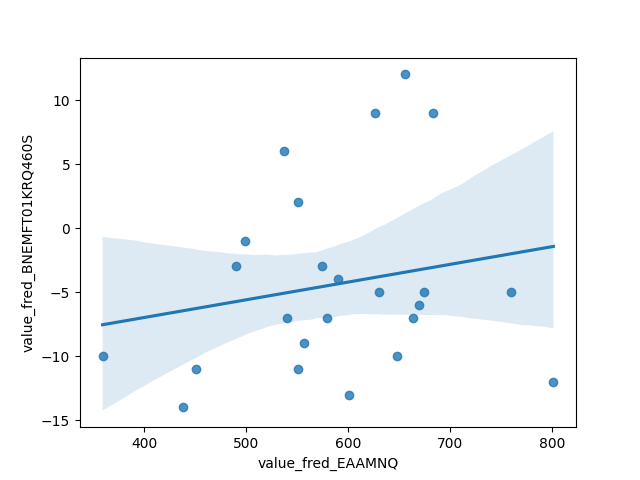
\includegraphics[scale = 0.9]{plots/plot_2025-01-24.png}
\caption{Regression Plot for 2025-01-24}
\end{figure}
\newpage

\include{tex_things/day_2025-01-25}
\include{tex_things/day_2025-01-26}
\include{tex_things/day_2025-01-27}

\end{document}
